\documentclass{bredelebeamer}

\usepackage[T1]{fontenc}
\usepackage[scaled]{beramono}

\usepackage{color}
\definecolor{bluekeywords}{rgb}{0.13,0.13,1}
\definecolor{greencomments}{rgb}{0,0.5,0}
\definecolor{redstrings}{rgb}{0.9,0,0}

\usepackage{listings}
\lstset{language=[Sharp]C,
showspaces=false,
showtabs=false,
breaklines=true,
showstringspaces=false,
breakatwhitespace=true,
escapeinside={(*@}{@*)},
commentstyle=\color{greencomments},
keywordstyle=\color{bluekeywords}\bfseries,
stringstyle=\color{redstrings},
basicstyle=\ttfamily
}
\usepackage{geometry}
\usepackage{tikz}
\usepackage{hyperref}

\newcommand{\imagefolder}{../EF.Experiments/EF.Experiments.Data/Specifications/Specification.cs}
\tikzset{
    invisible/.style={opacity=0},
    visible on/.style={alt={#1{}{invisible}}},
    alt/.code args={<#1>#2#3}{%
      \alt<#1>{\pgfkeysalso{#2}}{\pgfkeysalso{#3}} % \pgfkeysalso doesn't change the path
    },
}

\usetikzlibrary{positioning,shadows,arrows}
\title[EFC Tips \& Tricks]{Entity Framework Core: Tips and Tricks}

% \subtitle{Some subtitle}

\author{Eduard Lepner\inst{1}}
\institute[Powel]
{
  \inst{1}%
  Powel AS\\
  Team Leader at Powel Water
  }


\date{12 April 2018}

\subject{EF Core: Tips and Tricks}
% Goes to PDF Metadata

\logo{

\includegraphics[scale=0.10]{images/logo.jpg}
}

\begin{document}

\begin{frame}
  \titlepage
\end{frame}

\begin{frame}{Agenda}
  \tableofcontents
\end{frame}

\section{Theory}
\subsection{EF Basic Primitives}
\begin{frame} {About Entity Framework}
    \begin{columns}[t]
        \begin{column}{0.5\textwidth}
            Queries\\[.2cm]
            \begin{enumerate}
                \item Queries (Where clauses, Take, Skip, OrderBy)
                \item Projections (Select statement)
                \item Aggregate (Min, Max, GroupBy)
            \end{enumerate}
            \onslide<2->{
                \begin{itemize}
                    \item Expression analysis
                    \item Expression translations
                    \item SQL Builder
                \end{itemize}
            }
            
        \end{column}
        \begin{column}{0.5\textwidth}
            Commands\\[.2cm]
            \begin{enumerate}
                \item Create
                \item Read
                \item Update
                \item Delete
            \end{enumerate}
            \onslide<3->{
                    \begin{itemize}
                        \item Dynamic Proxies
                        \item Changes Detection (Object graph tracking)
                    \end{itemize}
                }
        \end{column}
    \end{columns}
\end{frame}
\subsection{Expression and Abstract Syntax Trees}
\begin{frame}{Expression Trees}
    \begin{block}{Any valid OO, Procedural, Declarative or Functional code}
        can be translated to an Abstract Syntax Tree (AST)...
        \pause  ... aaaand vice versa
    \end{block}
    \pause
    \begin{block}{AST}
        is a language indepent abstraction \pause (that's why FP is cool)
    \end{block}
    \pause
    \begin{block}{Expression Tree}
        is an AST. Expression yields one value and AST may represent entire program
    \end{block}
    
    \begin{alertblock}{Bingo!}
        Language A $\Rightarrow$ AST $\Rightarrow$ Language B
    \end{alertblock}
\end{frame}
\subsection{C\# Language Primitives and Syntax Sugar}
\begin{frame}[fragile]{Simple State}
    \begin{lstlisting}
var query = dbContext.Posts
    .Where(x => x.Content.StartsWith("Some") || x.Title.Length > 10)
    .Select(x => new { x.Id, x.Title, x.Content })
    \end{lstlisting}
    \pause
    \begin{lstlisting}
var query2 = Queryable.Select(
    Queryable.Where(
        dbContext.Posts, x => x.Content.StartsWith("Some") || x.Title.Length > 10),
    x => new { x.Id, x.Title, x.Content })
    \end{lstlisting}
\end{frame}

\begin{frame}[fragile]{C\# Syntax Sugar}
    \begin{onlyenv}<1>
        \begin{lstlisting}
        var query = from ac in _context.AddressConnection
            join cp in _context.ConsumptionPlace on ac.AddressObjectID equals cp.Id
            join cc in _context.CustomerConnection on cp.Id equals cc.CustomerObjectID
            join cu in _context.Customer on cc.CustomerID equals cu.Id
            where ac.AddressObjectTable == nameof(ConsumptionPlace) && ac.AddressID == id &&
            cc.CustomerObjectTable == nameof(ConsumptionPlace) && cc.CustomerRoleCode == CustomerRoleCodes.Consumer
            select new ViewModels.ConsumptionPlacePanelView
            {
                Id = cp.Id,
                Name = cu.Name
            };
        \end{lstlisting}
    \end{onlyenv}
    \begin{onlyenv}<2>
        \begin{lstlisting}
        var query = _context.AddressConnection
            .Join(_context.ConsumptionPlace, ac => ac.AddressObjectID, cp => cp.Id, (ac, cp) => new {ac, cp})
            .Join(_context.CustomerConnection, t => t.cp.Id, cc => cc.CustomerObjectID, (t, cc) => new {t, cc})
            .Join(_context.Customer, t => t.cc.CustomerID, cu => cu.Id, (t, cu) => new {t, cu})
            .Where(t => t.t.t.ac.AddressObjectTable == nameof(ConsumptionPlace) && t.t.t.ac.AddressID == id &&
                         t.t.cc.CustomerObjectTable == nameof(ConsumptionPlace) &&
                         t.t.cc.CustomerRoleCode == CustomerRoleCodes.Consumer)
            .Select(t => new ViewModels.ConsumptionPlacePanelView {Id = t.t.t.cp.Id, Name = t.cu.Name});
        \end{lstlisting}
    \end{onlyenv}
\end{frame}
\begin{frame}{IEnumerable<T> vs IQueryble<T>}
    \lstinline{DbSet<T>} implements both \lstinline{IEnumerable<T>} and \lstinline{IQueryble<T>}.
    How does it know which \lstinline{Select, Where, FirstOrDefault} to use?
    \pause
    \begin{block}{7.5.3.5 Better conversion target}
        Given two different types T1 and T2, T1 is a better conversion target than T2 if at least one of the following holds:
        \begin{itemize}
            \item An implicit conversion from T1 to T2 exists, and no implicit conversion from T2 toT1 exists
            \item T1 is a signed integral type and T2 is an unsigned integral type.
        \end{itemize}
    \end{block}
    \begin{exampleblock}{Lambda Expressions}
        A lambda expression is an anonymous function that you can use to create delegates or expression tree types. By using lambda expressions, you can write local functions that can be passed as arguments or returned as the value of function calls.
    \end{exampleblock}
\end{frame}
\subsection{Expression Parsing}
\begin{frame}[fragile]{Expression Parsing}
    \begin{lstlisting}
dbContext.Posts.Where(x => x.Content.StartsWith("Some") || x.Title.Length > 10).Select(x => new { x.Id, x.Title, x.Content })
    \end{lstlisting}
    \pause
    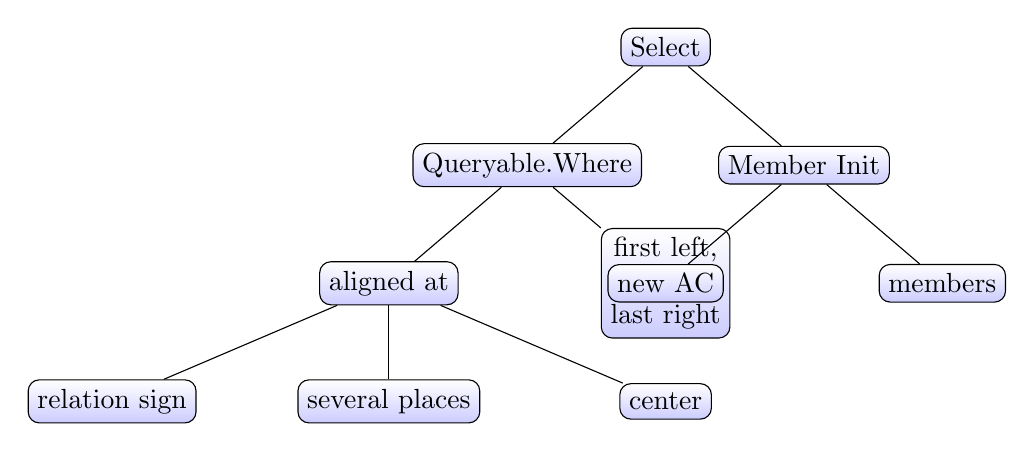
\begin{tikzpicture}[sibling distance=10em,
    every node/.style = {shape=rectangle, rounded corners,
      draw, align=center,
      top color=white, bottom color=blue!20}]]
    \node {Select}
        % child { node {single-line} }
        child { node {Queryable.Where}
        child { node {aligned at}
            child { node {relation sign} }
            child { node {several places} }
            child { node {center} } }
        child { node {first left,\\centered,\\last right} } }
        child {node {Member Init}
            child { node {new AC} }
            child { node {members} } };
\end{tikzpicture}
\end{frame}
\subsection*{Conclusions}
\begin{frame}[fragile]{Conclusions}
    \begin{itemize}
        \item<1-> EF is not magic
        \item<2-> One can pass around Query object append/modify it's nodes (aka Where/Select/OrderBy)
        \item<3-> { This code is not equivalent
        \begin{columns}
            \begin{column}{0.5\textwidth}
                \begin{lstlisting}
new Clazz{A = "A", B = "B"}
                \end{lstlisting}
            \end{column}
            \begin{column}{0.5\textwidth}
                \begin{lstlisting}
var c = new Clazz();
c.A = "A";
c.B = "B";
                \end{lstlisting}
            \end{column}
        \end{columns}
        }
    \end{itemize}
\end{frame}

\section{Level Easy}
\subsection{ViewModel Projectsions}
\begin{frame}{Projection (ViewModels)}
    \begin{onlyenv}<1>
        \lstinputlisting{resources/model.cs}
    \end{onlyenv}
    \begin{onlyenv}<2>
        \lstinputlisting{resources/viewmodel.cs}
    \end{onlyenv}
\end{frame}

\begin{frame}[fragile]{Projections}
    \begin{onlyenv}<1>
        \begin{lstlisting}
var query = dbContext.Authors.Include(x => x.Posts).Select(x => new ViewModels.Author
{
    Id = x.Id,
    Name = x.Name + " " + x.LastName,
}).Where(authorView => authorView.Id != 5)
        \end{lstlisting}
    \end{onlyenv}
    \begin{onlyenv}<2>
        \begin{lstlisting}
var query = dbContext.Authors.Include(x => x.Posts).Select(x => new ViewModels.Author
        {
            Id = x.Id,
            Name = x.Name + " " + x.LastName,
            Posts = x.Posts.Select(y => y.Id).ToList()
        }).Where(authorView => authorView.Id != 5)
                .OrderBy(autoryView => autoryView.Name)
    .ToArray();
        \end{lstlisting}
        \begin{alertblock}{Important}
            Nested property translation only after EFC 2.1.0-preview1
        \end{alertblock}
    \end{onlyenv}
\end{frame}
\begin{frame}[fragile]{Projections (SQL Result)}
    \begin{lstlisting}[language=SQL]
        SELECT [t].[c], [t].[Id], [t].[Name], [t].[LastName], [x.Posts].[Id], [x.Posts].[AuthorId]
        FROM [Posts] AS [x.Posts]
        INNER JOIN (
            SELECT ([x0].[Name] + N' ') + [x0].[LastName] AS [c], [x0].[Id], [x0].[Name], [x0].[LastName]
            FROM [Authors] AS [x0]
            WHERE [x0].[Id] <> 5
        ) AS [t] ON [x.Posts].[AuthorId] = [t].[Id]
        ORDER BY [t].[c], [t].[Id]
    \end{lstlisting}
\end{frame}
\subsection{à la C\# Triggers}
\begin{frame}{C\# Triggers}
    \lstinputlisting[firstline=47, lastline=59]{../EF.Experiments/EF.Experiments.Data/BloggingContext.cs}
    \pause
    Don't forget to override Async verion of SaveChanges on EF Core.

\end{frame}
\subsection{Object Tracking}
\begin{frame}{Object Tracking}
    \lstinputlisting[firstline=31, lastline=33]{../EF.Experiments/EF.Experiments/Program.cs}
    \pause
    \begin{exampleblock}{}
        True
    \end{exampleblock}
\end{frame}

\begin{frame}{What if I Don't Want To Track}
    \begin{exampleblock}{}
        Use AsNoTracking() method
    \end{exampleblock}{}
\end{frame}

\section{Medium Level}
\subsection{Avoiding N+1 Problem}
\begin{frame}{Tracking N+1 Problem}
    \begin{alertblock}{N+1 Fallback}
        Unlike EF6, if EFC cannot translate expression it will execute it on client.
    \end{alertblock}
    \pause
    \begin{exampleblock}{Treat Warnings as Errors}
        optionsBuilder\\
                .UseSqlServer(...)\\
                .ConfigureWarnings(wartings => wartings.Throw());
    \end{exampleblock}
\end{frame}
\subsection{Pattern Specification}
\begin{frame}[fragile]{Pattern Specification}
    \begin{block}{Specification}
        In computer programming, the specification pattern is a particular software design pattern, whereby business rules can be recombined by chaining the business rules together using boolean logic. 
    \end{block}
    \pause
    \begin{lstlisting}
        public interface ISpecification<T>
        {
            bool IsSatisfiedBy(T entity);
    \end{lstlisting}
    \pause
    \begin{lstlisting}
            Expression<Func<T, bool>> ToExpression();
        }
    \end{lstlisting}
\end{frame}
\begin{frame}[fragile]{Now We Can}
    \lstinputlisting[firstline=8, lastline=21]{../EF.Experiments/EF.Experiments.Data/Specifications/Implementations/Implementations.cs}
\end{frame}

\begin{frame}[fragile]{Now We Can}
    \begin{lstlisting}
context.Posts.Where(new LastPosts(10).ToExpression())
    \end{lstlisting}
    \begin{itemize}
        \item{Testable}
        \item{Incapsulate Business logic}
    \end{itemize}
\end{frame}
\section{Advanced}
\subsection{Advanced Pattern Specification}
\begin{frame}{But Specification Pattern says they should be capable of chaining}
    
\includegraphics[scale=0.8]{images/But.png}
\end{frame}
\begin{frame}[fragile]{Goal}
    \begin{itemize}[<+->]
        \item {
            No Explicit ToExpression() calls/Casts
            \begin{lstlisting}
    ctx.Posts.Where(new LastPosts(10))
            \end{lstlisting}
        }
        \item {
            Linq To Enities
            \begin{lstlisting}
    ctx.Posts.ToArray().Where(new LastPosts(10))
            \end{lstlisting}
        }
        \item {
            Chaining with boolean operators?
            \begin{lstlisting}
    ctx.Posts.ToArray().Where(
        new LastPosts(10) && new FromBlog(blogId) &&
            (new ByAuthor(john) || new ByAuthor(Grzegosz))
        )
            \end{lstlisting}
        }
    \end{itemize}

\end{frame}
\begin{frame}{Can we achieve this with C\#?}
    \pause
    \begin{center}
        \huge What if I told you it was possible?
        
\includegraphics[scale=0.45]{images/whatifitoldyou.jpg}
    \end{center}
\end{frame}
% \def\spec_file_path {../EF.Experiments/EF.Experiments.Data/Specifications/Specification.cs}

\begin{frame}[fragile]{Reaching our Goal With Specification Pattern}
    \begin{itemize}[<+->]
        \item {
            No Explicit ToExpression() calls/Casts - operator overloading
        }
        \item {
            Linq To Enities
        }
        \item {
            Chaining with boolean operators
        }
    \end{itemize}
    \only<1> {
        \lstinputlisting[firstline=37, lastline=40]{\imagefolder}
    }
    \only<2> {
        \lstinputlisting[firstline=10, lastline=11]{\imagefolder}
        \lstinputlisting[firstline=32, lastline=35]{\imagefolder}
    }
    \only<3> {
        \begin{block}{\href{https://docs.microsoft.com/en-us/dotnet/csharp/language-reference/language-specification/expressions\#boolean-expressions}{Boolean operator overloading}}
            In order to overloading operators \&\&, ||, ! one should overload operators true, false, \&, |
        \end{block}
        CODE DEMO!
    }
\end{frame}
\subsection{EFC DI Model}
\begin{frame}{DI in EFC}
    \begin{itemize}[<+->]
        \item EFC uses the same approach with IServiceCollection as ASP.NET Core does
        \item One can replace any service with one's own implementstion using DbContextOptionsBuilder.ReplaceService
        \item Extension methods like DbContextOptionsBuilder.Use...() set up necessary services like UseMvc() in AspNet.Core
    \end{itemize}
\end{frame}
\begin{frame}{EFC DI Model Example}
    One can look at example in \href{https://github.com/aspnet/EntityFrameworkCore/blob/dev/src/EFCore.SqlServer/Extensions/SqlServerServiceCollectionExtensions.cs}{SqlServerServiceCollectionExtensions.cs}
    and \href{https://github.com/aspnet/EntityFrameworkCore/blob/dev/src/EFCore/Infrastructure/EntityFrameworkServicesBuilder.cs}{EntityFrameworkServicesBuilder.cs}.

    They add about 100 services to IServiceCollection
\end{frame}
\subsection{Custom SQL Operator}
\begin{frame}[fragile]{Implementing Custom SQL Operator}
    \begin{enumerate}[<+->]
        \item {
            Goal: SQL Query like this:
            \begin{lstlisting}[language=SQL]
    SELECT * FROM Posts WHERE CONTAINS(content, N'some text')
            \end{lstlisting}
        }
        \item {
            Produced from like that:
            \begin{lstlisting}[language=SQL]
    dbContext.Posts.Where(x => !x.Content.ContainsText("some text"))
            \end{lstlisting}
        }
    \end{enumerate}
\end{frame}
\begin{frame}[fragile]{CONTAINS Operator Implementaion (Translator)}
    \begin{lstlisting}
public class FreeTextTranslator : IMethodCallTranslator
{
    private static readonly MethodInfo _methodInfo
        = typeof(StringExt).GetRuntimeMethod(nameof(StringExt.ContainsText), new[] {typeof(string), typeof(string)});

    public Expression Translate(MethodCallExpression methodCallExpression)
    {
        if (methodCallExpression.Method != _methodInfo) return null;

        var patternExpression = methodCallExpression.Arguments[1];
        var objectExpression = (ColumnExpression) methodCallExpression.Arguments[0];

        var sqlExpression =
            new SqlFunctionExpression("CONTAINS", typeof(bool),
                new[] { objectExpression, patternExpression });
        return sqlExpression;
    }
}
    \end{lstlisting}
\end{frame}

\begin{frame}[fragile]{CONTAINS Operator Implementaion (Appending to DI pipeline)}
    \begin{lstlisting}
public class CustomSqlMethodCallTranslator : SqlServerCompositeMethodCallTranslator
{
    public CustomSqlMethodCallTranslator(RelationalCompositeMethodCallTranslatorDependencies dependencies) : base(dependencies)
    {
        // ReSharper disable once VirtualMemberCallInConstructor
        AddTranslators(new [] {new FreeTextTranslator() });
    }
}
    \end{lstlisting}
    \href{https://github.com/aspnet/EntityFrameworkCore/blob/dev/src/EFCore.SqlServer/Query/ExpressionTranslators/Internal/SqlServerCompositeMethodCallTranslator.cs}{SqlServerCompositeMethodCallTranslator.cs}
    \href{https://github.com/aspnet/EntityFrameworkCore/blob/dev/src/EFCore.Relational/Query/ExpressionTranslators/RelationalCompositeMethodCallTranslator.cs\#L56}{RelationalCompositeMethodCallTranslator.cs}

    \begin{lstlisting}
optionsBuilder.ReplaceService<ICompositeMethodCallTranslator, CustomSqlMethodCallTranslator>();
    \end{lstlisting}
\end{frame}

\begin{frame}[fragile]{Problems with boolean function}
    \begin{block}{}
        Because of this \href{https://github.com/aspnet/EntityFrameworkCore/issues/11316}{\#11316} and that \href{https://github.com/aspnet/EntityFrameworkCore/issues/9143}{\#9143}
        EFC does not recoginze bool type of SqlFunction (predicate) and produce invalid SQL
    \end{block}
    \begin{lstlisting}[language=SQL]
    SELECT [x].[Id], [x].[AuthorId], [x].[BlogId], [x].[Content], [x].[Created], [x].[Rating], [x].[Title]
        FROM [Posts] AS [x]
        WHERE CONTAINS([x].[Content], N'some text') = 1
    \end{lstlisting}
\end{frame}
\begin{frame}[fragile]{Fixing "= 1" Problem}
    \lstinputlisting[firstline=7, lastline=25]{../EF.Experiments/EF.Experiments.Data/FreeTextSqlGenerator.cs}
\end{frame}
\section*{Final}
\begin{frame}{Thank you for listening!}
    Links:
    \begin{itemize}
        \item{
            Project: \href{https://github.com/elepner/ef-experiments}{https://github.com/elepner/ef-experiments}
        }
        \item{
            Presentation: \href{https://github.com/elepner/ef.presentation}{https://github.com/elepner/ef.presentation}
        }
        \item{
            Entity Framework Core Project: \href{https://github.com/aspnet/EntityFrameworkCore}{https://github.com/aspnet/EntityFrameworkCore}
        }
    \end{itemize}
\end{frame}
\end{document}
